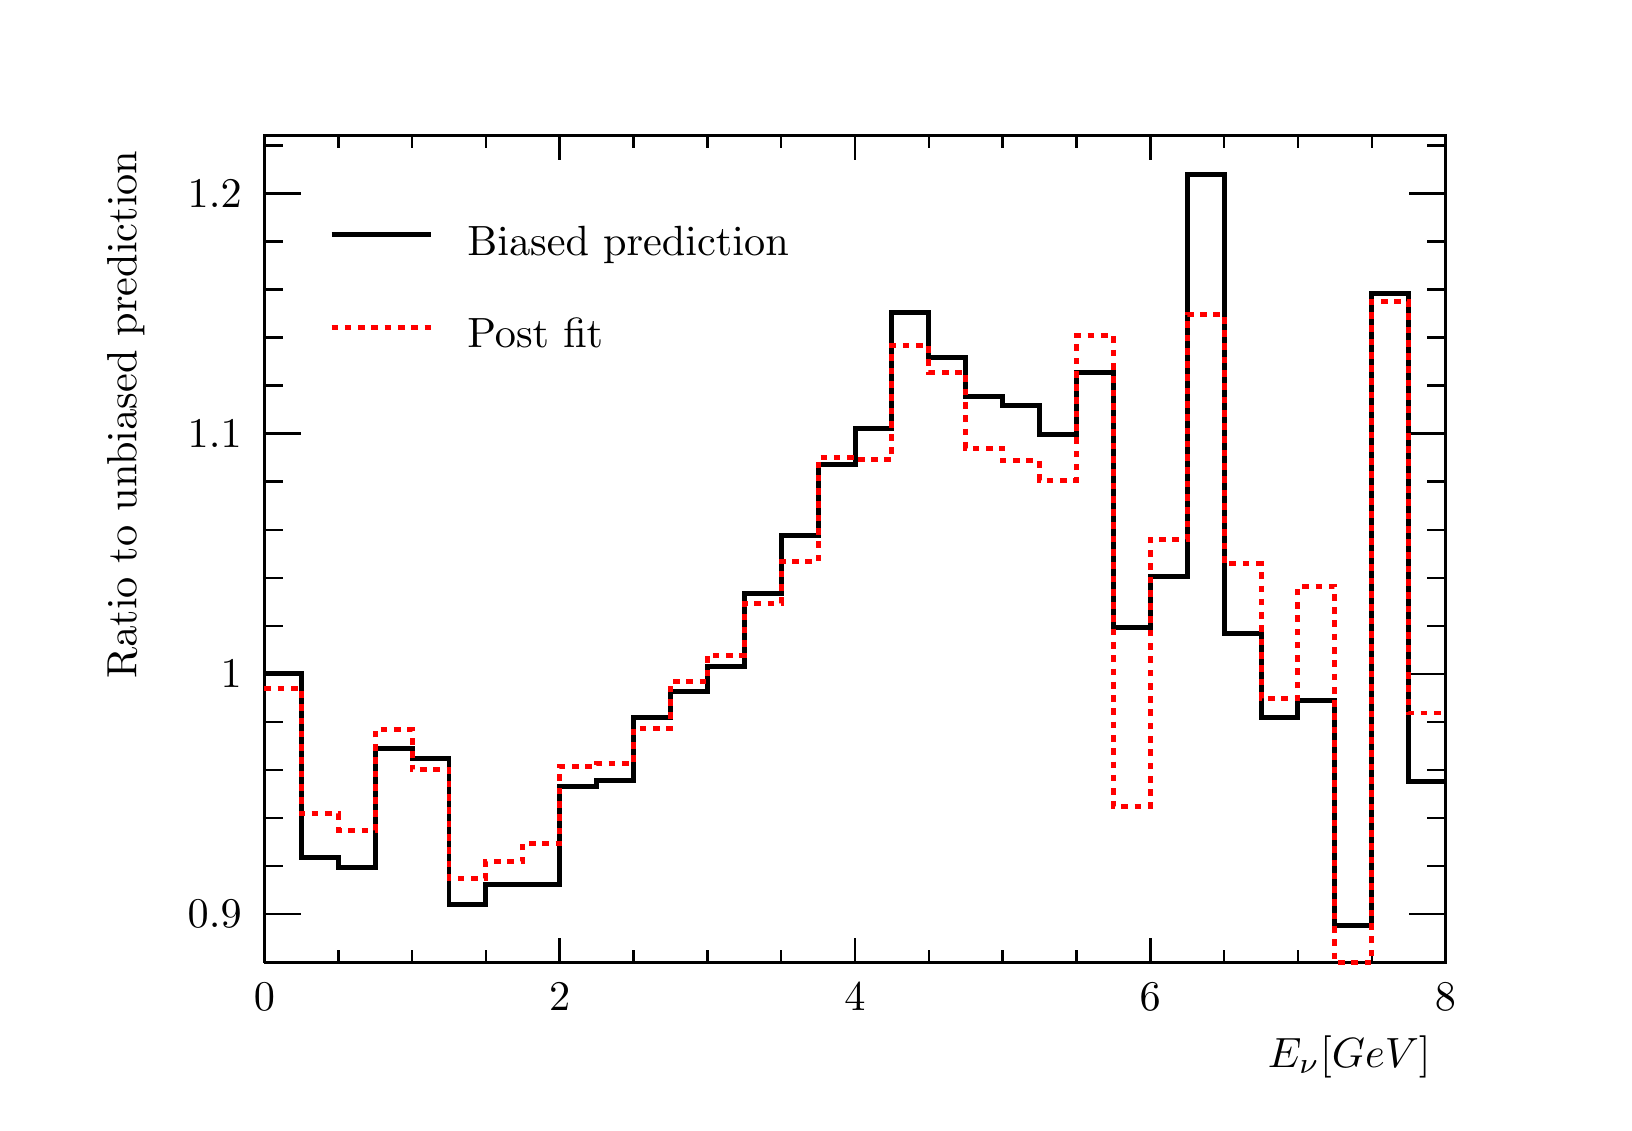
\begin{tikzpicture}
\pgfdeclareplotmark{cross} {
\pgfpathmoveto{\pgfpoint{-0.3\pgfplotmarksize}{\pgfplotmarksize}}
\pgfpathlineto{\pgfpoint{+0.3\pgfplotmarksize}{\pgfplotmarksize}}
\pgfpathlineto{\pgfpoint{+0.3\pgfplotmarksize}{0.3\pgfplotmarksize}}
\pgfpathlineto{\pgfpoint{+1\pgfplotmarksize}{0.3\pgfplotmarksize}}
\pgfpathlineto{\pgfpoint{+1\pgfplotmarksize}{-0.3\pgfplotmarksize}}
\pgfpathlineto{\pgfpoint{+0.3\pgfplotmarksize}{-0.3\pgfplotmarksize}}
\pgfpathlineto{\pgfpoint{+0.3\pgfplotmarksize}{-1.\pgfplotmarksize}}
\pgfpathlineto{\pgfpoint{-0.3\pgfplotmarksize}{-1.\pgfplotmarksize}}
\pgfpathlineto{\pgfpoint{-0.3\pgfplotmarksize}{-0.3\pgfplotmarksize}}
\pgfpathlineto{\pgfpoint{-1.\pgfplotmarksize}{-0.3\pgfplotmarksize}}
\pgfpathlineto{\pgfpoint{-1.\pgfplotmarksize}{0.3\pgfplotmarksize}}
\pgfpathlineto{\pgfpoint{-0.3\pgfplotmarksize}{0.3\pgfplotmarksize}}
\pgfpathclose
\pgfusepathqstroke
}
\pgfdeclareplotmark{cross*} {
\pgfpathmoveto{\pgfpoint{-0.3\pgfplotmarksize}{\pgfplotmarksize}}
\pgfpathlineto{\pgfpoint{+0.3\pgfplotmarksize}{\pgfplotmarksize}}
\pgfpathlineto{\pgfpoint{+0.3\pgfplotmarksize}{0.3\pgfplotmarksize}}
\pgfpathlineto{\pgfpoint{+1\pgfplotmarksize}{0.3\pgfplotmarksize}}
\pgfpathlineto{\pgfpoint{+1\pgfplotmarksize}{-0.3\pgfplotmarksize}}
\pgfpathlineto{\pgfpoint{+0.3\pgfplotmarksize}{-0.3\pgfplotmarksize}}
\pgfpathlineto{\pgfpoint{+0.3\pgfplotmarksize}{-1.\pgfplotmarksize}}
\pgfpathlineto{\pgfpoint{-0.3\pgfplotmarksize}{-1.\pgfplotmarksize}}
\pgfpathlineto{\pgfpoint{-0.3\pgfplotmarksize}{-0.3\pgfplotmarksize}}
\pgfpathlineto{\pgfpoint{-1.\pgfplotmarksize}{-0.3\pgfplotmarksize}}
\pgfpathlineto{\pgfpoint{-1.\pgfplotmarksize}{0.3\pgfplotmarksize}}
\pgfpathlineto{\pgfpoint{-0.3\pgfplotmarksize}{0.3\pgfplotmarksize}}
\pgfpathclose
\pgfusepathqfillstroke
}
\pgfdeclareplotmark{newstar} {
\pgfpathmoveto{\pgfqpoint{0pt}{\pgfplotmarksize}}
\pgfpathlineto{\pgfqpointpolar{44}{0.5\pgfplotmarksize}}
\pgfpathlineto{\pgfqpointpolar{18}{\pgfplotmarksize}}
\pgfpathlineto{\pgfqpointpolar{-20}{0.5\pgfplotmarksize}}
\pgfpathlineto{\pgfqpointpolar{-54}{\pgfplotmarksize}}
\pgfpathlineto{\pgfqpointpolar{-90}{0.5\pgfplotmarksize}}
\pgfpathlineto{\pgfqpointpolar{234}{\pgfplotmarksize}}
\pgfpathlineto{\pgfqpointpolar{198}{0.5\pgfplotmarksize}}
\pgfpathlineto{\pgfqpointpolar{162}{\pgfplotmarksize}}
\pgfpathlineto{\pgfqpointpolar{134}{0.5\pgfplotmarksize}}
\pgfpathclose
\pgfusepathqstroke
}
\pgfdeclareplotmark{newstar*} {
\pgfpathmoveto{\pgfqpoint{0pt}{\pgfplotmarksize}}
\pgfpathlineto{\pgfqpointpolar{44}{0.5\pgfplotmarksize}}
\pgfpathlineto{\pgfqpointpolar{18}{\pgfplotmarksize}}
\pgfpathlineto{\pgfqpointpolar{-20}{0.5\pgfplotmarksize}}
\pgfpathlineto{\pgfqpointpolar{-54}{\pgfplotmarksize}}
\pgfpathlineto{\pgfqpointpolar{-90}{0.5\pgfplotmarksize}}
\pgfpathlineto{\pgfqpointpolar{234}{\pgfplotmarksize}}
\pgfpathlineto{\pgfqpointpolar{198}{0.5\pgfplotmarksize}}
\pgfpathlineto{\pgfqpointpolar{162}{\pgfplotmarksize}}
\pgfpathlineto{\pgfqpointpolar{134}{0.5\pgfplotmarksize}}
\pgfpathclose
\pgfusepathqfillstroke
}
\definecolor{c}{rgb}{1,1,1};
\draw [color=c, fill=c] (0,0) rectangle (20,13.639);
\draw [color=c, fill=c] (3,1.77307) rectangle (18,12.2751);
\definecolor{c}{rgb}{0,0,0};
\draw [c,line width=0.9] (3,1.77307) -- (3,12.2751) -- (18,12.2751) -- (18,1.77307) -- (3,1.77307);
\definecolor{c}{rgb}{1,1,1};
\draw [color=c, fill=c] (3,1.77307) rectangle (18,12.2751);
\definecolor{c}{rgb}{0,0,0};
\draw [c,line width=0.9] (3,1.77307) -- (3,12.2751) -- (18,12.2751) -- (18,1.77307) -- (3,1.77307);
\draw [c,line width=1.8] (3,5.4398) -- (3.46875,5.4398) -- (3.46875,3.11046) -- (3.9375,3.11046) -- (3.9375,2.9847) -- (4.40625,2.9847) -- (4.40625,4.49628) -- (4.875,4.49628) -- (4.875,4.35994) -- (5.34375,4.35994) -- (5.34375,2.51098) --
 (5.8125,2.51098) -- (5.8125,2.76854) -- (6.28125,2.76854) -- (6.28125,2.76909) -- (6.75,2.76909) -- (6.75,4.00843) -- (7.21875,4.00843) -- (7.21875,4.07905) -- (7.6875,4.07905) -- (7.6875,4.8814) -- (8.15625,4.8814) -- (8.15625,5.211) --
 (8.625,5.211) -- (8.625,5.53438) -- (9.09375,5.53438) -- (9.09375,6.46036) -- (9.5625,6.46036) -- (9.5625,7.19297) -- (10.0312,7.19297) -- (10.0312,8.09512) -- (10.5,8.09512) -- (10.5,8.56119) -- (10.9688,8.56119) -- (10.9688,10.0267) --
 (11.4375,10.0267) -- (11.4375,9.45988) -- (11.9062,9.45988) -- (11.9062,8.96634) -- (12.375,8.96634) -- (12.375,8.85033) -- (12.8438,8.85033) -- (12.8438,8.47732) -- (13.3125,8.47732) -- (13.3125,9.2674) -- (13.7812,9.2674) -- (13.7812,6.02401) --
 (14.25,6.02401) -- (14.25,6.67724) -- (14.7188,6.67724) -- (14.7188,11.775) -- (15.1875,11.775) -- (15.1875,5.94879) -- (15.6562,5.94879) -- (15.6562,4.891) -- (16.125,4.891) -- (16.125,5.10081) -- (16.5938,5.10081) -- (16.5938,2.24935) --
 (17.0625,2.24935) -- (17.0625,10.2758) -- (17.5312,10.2758) -- (17.5312,4.06917) -- (18,4.06917);
\draw [c,line width=0.9] (3,1.77307) -- (18,1.77307);
\draw [c,line width=0.9] (3,2.07994) -- (3,1.77307);
\draw [c,line width=0.9] (3.9375,1.9265) -- (3.9375,1.77307);
\draw [c,line width=0.9] (4.875,1.9265) -- (4.875,1.77307);
\draw [c,line width=0.9] (5.8125,1.9265) -- (5.8125,1.77307);
\draw [c,line width=0.9] (6.75,2.07994) -- (6.75,1.77307);
\draw [c,line width=0.9] (7.6875,1.9265) -- (7.6875,1.77307);
\draw [c,line width=0.9] (8.625,1.9265) -- (8.625,1.77307);
\draw [c,line width=0.9] (9.5625,1.9265) -- (9.5625,1.77307);
\draw [c,line width=0.9] (10.5,2.07994) -- (10.5,1.77307);
\draw [c,line width=0.9] (11.4375,1.9265) -- (11.4375,1.77307);
\draw [c,line width=0.9] (12.375,1.9265) -- (12.375,1.77307);
\draw [c,line width=0.9] (13.3125,1.9265) -- (13.3125,1.77307);
\draw [c,line width=0.9] (14.25,2.07994) -- (14.25,1.77307);
\draw [c,line width=0.9] (15.1875,1.9265) -- (15.1875,1.77307);
\draw [c,line width=0.9] (16.125,1.9265) -- (16.125,1.77307);
\draw [c,line width=0.9] (17.0625,1.9265) -- (17.0625,1.77307);
\draw [c,line width=0.9] (18,2.07994) -- (18,1.77307);
\draw [anchor=base] (3,1.15931) node[scale=1.52731, color=c, rotate=0]{0};
\draw [anchor=base] (6.75,1.15931) node[scale=1.52731, color=c, rotate=0]{2};
\draw [anchor=base] (10.5,1.15931) node[scale=1.52731, color=c, rotate=0]{4};
\draw [anchor=base] (14.25,1.15931) node[scale=1.52731, color=c, rotate=0]{6};
\draw [anchor=base] (18,1.15931) node[scale=1.52731, color=c, rotate=0]{8};
\draw [anchor= east] (18,0.572837) node[scale=1.52731, color=c, rotate=0]{$E_{\nu} [GeV]$};
\draw [c,line width=0.9] (3,12.2751) -- (18,12.2751);
\draw [c,line width=0.9] (3,11.9682) -- (3,12.2751);
\draw [c,line width=0.9] (3.9375,12.1216) -- (3.9375,12.2751);
\draw [c,line width=0.9] (4.875,12.1216) -- (4.875,12.2751);
\draw [c,line width=0.9] (5.8125,12.1216) -- (5.8125,12.2751);
\draw [c,line width=0.9] (6.75,11.9682) -- (6.75,12.2751);
\draw [c,line width=0.9] (7.6875,12.1216) -- (7.6875,12.2751);
\draw [c,line width=0.9] (8.625,12.1216) -- (8.625,12.2751);
\draw [c,line width=0.9] (9.5625,12.1216) -- (9.5625,12.2751);
\draw [c,line width=0.9] (10.5,11.9682) -- (10.5,12.2751);
\draw [c,line width=0.9] (11.4375,12.1216) -- (11.4375,12.2751);
\draw [c,line width=0.9] (12.375,12.1216) -- (12.375,12.2751);
\draw [c,line width=0.9] (13.3125,12.1216) -- (13.3125,12.2751);
\draw [c,line width=0.9] (14.25,11.9682) -- (14.25,12.2751);
\draw [c,line width=0.9] (15.1875,12.1216) -- (15.1875,12.2751);
\draw [c,line width=0.9] (16.125,12.1216) -- (16.125,12.2751);
\draw [c,line width=0.9] (17.0625,12.1216) -- (17.0625,12.2751);
\draw [c,line width=0.9] (18,11.9682) -- (18,12.2751);
\draw [c,line width=0.9] (3,1.77307) -- (3,12.2751);
\draw [c,line width=0.9] (3.462,2.39013) -- (3,2.39013);
\draw [c,line width=0.9] (3.231,3.00006) -- (3,3.00006);
\draw [c,line width=0.9] (3.231,3.61) -- (3,3.61);
\draw [c,line width=0.9] (3.231,4.21993) -- (3,4.21993);
\draw [c,line width=0.9] (3.231,4.82986) -- (3,4.82986);
\draw [c,line width=0.9] (3.462,5.4398) -- (3,5.4398);
\draw [c,line width=0.9] (3.231,6.04973) -- (3,6.04973);
\draw [c,line width=0.9] (3.231,6.65966) -- (3,6.65966);
\draw [c,line width=0.9] (3.231,7.26959) -- (3,7.26959);
\draw [c,line width=0.9] (3.231,7.87953) -- (3,7.87953);
\draw [c,line width=0.9] (3.462,8.48946) -- (3,8.48946);
\draw [c,line width=0.9] (3.231,9.09939) -- (3,9.09939);
\draw [c,line width=0.9] (3.231,9.70933) -- (3,9.70933);
\draw [c,line width=0.9] (3.231,10.3193) -- (3,10.3193);
\draw [c,line width=0.9] (3.231,10.9292) -- (3,10.9292);
\draw [c,line width=0.9] (3.462,11.5391) -- (3,11.5391);
\draw [c,line width=0.9] (3.462,2.39013) -- (3,2.39013);
\draw [c,line width=0.9] (3.231,1.7802) -- (3,1.7802);
\draw [c,line width=0.9] (3.462,11.5391) -- (3,11.5391);
\draw [c,line width=0.9] (3.231,12.1491) -- (3,12.1491);
\draw [anchor= east] (2.9,2.39013) node[scale=1.52731, color=c, rotate=0]{0.9};
\draw [anchor= east] (2.9,5.4398) node[scale=1.52731, color=c, rotate=0]{1};
\draw [anchor= east] (2.9,8.48946) node[scale=1.52731, color=c, rotate=0]{1.1};
\draw [anchor= east] (2.9,11.5391) node[scale=1.52731, color=c, rotate=0]{1.2};
\draw [anchor= east] (1.24,12.2751) node[scale=1.52731, color=c, rotate=90]{Ratio to unbiased prediction};
\draw [c,line width=0.9] (18,1.77307) -- (18,12.2751);
\draw [c,line width=0.9] (17.538,2.39013) -- (18,2.39013);
\draw [c,line width=0.9] (17.769,3.00006) -- (18,3.00006);
\draw [c,line width=0.9] (17.769,3.61) -- (18,3.61);
\draw [c,line width=0.9] (17.769,4.21993) -- (18,4.21993);
\draw [c,line width=0.9] (17.769,4.82986) -- (18,4.82986);
\draw [c,line width=0.9] (17.538,5.4398) -- (18,5.4398);
\draw [c,line width=0.9] (17.769,6.04973) -- (18,6.04973);
\draw [c,line width=0.9] (17.769,6.65966) -- (18,6.65966);
\draw [c,line width=0.9] (17.769,7.26959) -- (18,7.26959);
\draw [c,line width=0.9] (17.769,7.87953) -- (18,7.87953);
\draw [c,line width=0.9] (17.538,8.48946) -- (18,8.48946);
\draw [c,line width=0.9] (17.769,9.09939) -- (18,9.09939);
\draw [c,line width=0.9] (17.769,9.70933) -- (18,9.70933);
\draw [c,line width=0.9] (17.769,10.3193) -- (18,10.3193);
\draw [c,line width=0.9] (17.769,10.9292) -- (18,10.9292);
\draw [c,line width=0.9] (17.538,11.5391) -- (18,11.5391);
\draw [c,line width=0.9] (17.538,2.39013) -- (18,2.39013);
\draw [c,line width=0.9] (17.769,1.7802) -- (18,1.7802);
\draw [c,line width=0.9] (17.538,11.5391) -- (18,11.5391);
\draw [c,line width=0.9] (17.769,12.1491) -- (18,12.1491);
\definecolor{c}{rgb}{1,0,0};
\draw [c,dash pattern=on 2.40pt off 2.40pt ,line width=1.8] (3,5.25944) -- (3.46875,5.25944) -- (3.46875,3.66623) -- (3.9375,3.66623) -- (3.9375,3.45604) -- (4.40625,3.45604) -- (4.40625,4.73163) -- (4.875,4.73163) -- (4.875,4.21864) --
 (5.34375,4.21864) -- (5.34375,2.84292) -- (5.8125,2.84292) -- (5.8125,3.05614) -- (6.28125,3.05614) -- (6.28125,3.28706) -- (6.75,3.28706) -- (6.75,4.25937) -- (7.21875,4.25937) -- (7.21875,4.30124) -- (7.6875,4.30124) -- (7.6875,4.74912) --
 (8.15625,4.74912) -- (8.15625,5.33804) -- (8.625,5.33804) -- (8.625,5.677) -- (9.09375,5.677) -- (9.09375,6.32992) -- (9.5625,6.32992) -- (9.5625,6.86214) -- (10.0312,6.86214) -- (10.0312,8.18887) -- (10.5,8.18887) -- (10.5,8.15668) --
 (10.9688,8.15668) -- (10.9688,9.61098) -- (11.4375,9.61098) -- (11.4375,9.26675) -- (11.9062,9.26675) -- (11.9062,8.3071) -- (12.375,8.3071) -- (12.375,8.14305) -- (12.8438,8.14305) -- (12.8438,7.89517) -- (13.3125,7.89517) -- (13.3125,9.73518) --
 (13.7812,9.73518) -- (13.7812,3.75201) -- (14.25,3.75201) -- (14.25,7.15177) -- (14.7188,7.15177) -- (14.7188,10.0055) -- (15.1875,10.0055) -- (15.1875,6.83543) -- (15.6562,6.83543) -- (15.6562,5.13074) -- (16.125,5.13074) -- (16.125,6.54894) --
 (16.5938,6.54894) -- (16.5938,1.77307) -- (17.0625,1.77307) -- (17.0625,10.1713) -- (17.5312,10.1713) -- (17.5312,4.94221) -- (18,4.94221);
\definecolor{c}{rgb}{1,1,1};
\draw [color=c, fill=c] (3.58166,9.25501) rectangle (10.8023,11.6046);
\definecolor{c}{rgb}{0,0,0};
\draw [anchor=base west] (5.38682,10.7529) node[scale=1.52731, color=c, rotate=0]{Biased prediction};
\draw [c,line width=1.8] (3.85244,11.0172) -- (5.11605,11.0172);
\draw [anchor=base west] (5.38682,9.57808) node[scale=1.52731, color=c, rotate=0]{Post fit};
\definecolor{c}{rgb}{1,0,0};
\draw [c,dash pattern=on 2.40pt off 2.40pt ,line width=1.8] (3.85244,9.84241) -- (5.11605,9.84241);
\end{tikzpicture}
